\chapter{Linear Least Square}

Nel capitolo precedente la risoluzione al problema Weighted Interval
Scheduling richiedeva una ricorsione basata su scelte
\textbf{\emph{binarie}}, in questo capitolo invece introdurremo un
algoritmo che richiede ad \textbf{\emph{ogni step un numero di scelte
    polinomiali}} (\emph{multi-way choice}). Vedremo come la programmazione
dinamica si presta molto bene a risolvere anche questo tipo di problemi.

\section{Descrizione del Problema}

\begin{myblockquote}
  Dato un insieme $P$ composto di $n$ punti sul piano denotati con \linebreak
  $(x_1, y_1), (x_2, y_2), \ldots, (x_n, y_n)$ e supponiamo che
  $x_1 < x_2 < \ldots < x_n$ (sono strettamente crescenti). Data una
  linea $L$ definita dall'equazione $y = ax + b$, definiamo
  l'\emph{errore} di $L$ in funzione di $P$ come la somma delle
  distanze al quadrato della linea rispetto ai punti in $P$.\\

  Formalmente:
  \begin{equation*}
    Error(L, P) = \sum_{i=1}^{n} (y_i - ax_i - b)^2
  \end{equation*}
\end{myblockquote}

\begin{figure}[H]
  \centering
  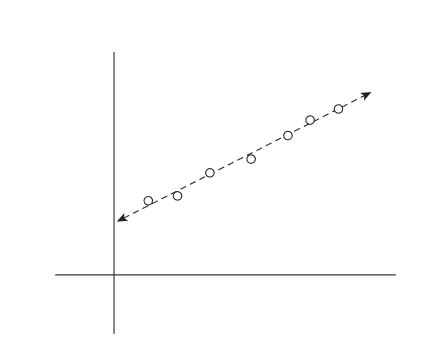
\includegraphics[width = 10cm, keepaspectratio]{capitoli/programmazione_dinamica/imgs/best_fit.png}
  \caption{Esempio di linea con errore minimo}
\end{figure}

\subsection{Goal}

Il goal dell'algoritmo è quello di \textbf{\emph{cercare la linea con
    errore minimo}}, che può essere facilmente trovata utilizzando
l'analisi matematica.\\

La linea di errore minimo è $y = ax + b$ dove:

$$
  a = \frac{n \sum_{i} x_i y_i - (\sum_{i} x_i) (\sum_{i} y_i)}{n \sum_{i} x_i^2 - (\sum_{i} x_i)^2} \ \ \  \ \ b = \frac{\sum_{i} y_i - a \sum_{i} x_i}{n}
$$

\section{Segmented Least Squares}

Le formule appena citate sono utilizzabili solo se i punti di $P$
hanno un andamento che è abbastanza lineare ma falliscono in altre
circostanze.

\begin{figure}[H]
  \centering
  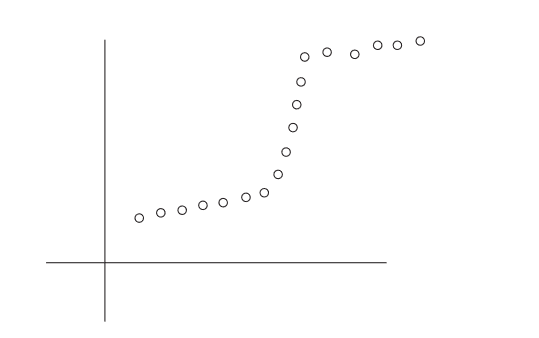
\includegraphics[width = 10cm, keepaspectratio]{capitoli/programmazione_dinamica/imgs/seg_llsqr.png}
  \caption{Esempio di insieme di punti non approssimabile con una sola retta}
\end{figure}

Come è evidente dalla figura non è possibile trovare una linea che
approssimi in maniera soddisfacente i punti, dunque per risolvere il
problema possiamo pensare di rilassare la condizione che sia solo una la
linea. Questo però implica dover riformulare il goal che altrimenti
risulterebbe banale (si fanno $n$ linee che passano per ogni punto).

\subsection{Goal}
Formalmente, il problema è espresso come segue:
\begin{myblockquote}
  Come prima abbiamo un set di punti
  $P = \{(x_1, y_1), (x_2, y_2), \ldots, (x_n, y_n)\}$ strettamente
  crescenti. Denoteremo l'insieme dei punti
  $(x_i, y_i)$ con $p_i$.\\
  Vogliamo partizionare $P$ in un qualche numero di segmenti, ogni numero di segmenti è un
  sottoinsieme di $P$ che rappresenta un \emph{set} contiguo delle
  coordinate $x$ con la forma
  $\{p_i, p_{i+1}, \ldots, p_{j-1}, p_j\}$ per degli indici
  $i \leq j$.\\
  Dopodiché, per ogni segmento $S$ calcoliamo la linea che minimizza l'errore rispetto ai punti in $S$
  secondo quanto espresso dalle formule enunciate prima.
\end{myblockquote}

Definiamo infine una \textbf{penalità} per una data partizione come la
somma dei seguenti termini:
\begin{itemize}
  \item Numero di segmenti in cui viene
        partizionato $P$ moltiplicato per un valore $C > 0$ (più è grande e
        più penalizza tante partizioni).
  \item Per ogni segmento l'errore della linea
        ottima attraverso quel segmento.
\end{itemize}

$$
  f(x) = E + C L
$$

Il goal del Segmented Least Square Problem è quindi quello di
\textbf{trovare la partizione di penalità minima}.

\section{Funzionamento}

Seguendo la logica alla base della programmazione dinamica, ci poniamo
l'obiettivo di suddividere il problema in sotto-problemi e, per farlo,
partiamo dall'osservazione che l'ultimo punto appartiene ad una
partizione ottima che parte da un valore $p_i$ fino a $p_n$ e che
possiamo togliere questi punti dal totale per ottenete un sotto-problema
più piccolo.
\begin{figure}[H]
  \centering
  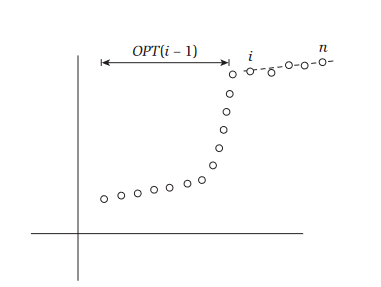
\includegraphics[width = 10cm, keepaspectratio]{capitoli/programmazione_dinamica/imgs/llsqr_funzionamento.png}
  \centering
  \caption{Una soluzione possibile per il fit digli ultimi punti da $p_i$ a $p_n$,
    e poi la soluzione $OPT(i-1)$ trovata nei punti rimanenti $p_1, \ldotp, p_{i-1}$}
\end{figure}
Supponiamo che la soluzione ottima sia denotata da
\texttt{OPT(j)}, per i punti che vanno da $p_1$ a $p_j$, allora
avremo che la soluzione ottima al problema dato l'ultimo segmento che va
da $p_i$ a $p_n$, sarà dalla seguente formula:

$$
  OPT(n) = e(i,n) + C + OPT(i - 1)
$$

Questa formula è data dalla soluzione ottima dell'ultima partizione ($e(i,n) +
  C$) a cui viene aggiunta la soluzione ottima di tutte le partizioni precedenti
($OPT(i -1)$).\\

Per i sotto-problemi possiamo scrivere la soluzione al problema in forma
ricorsiva utilizzando la formula appena espressa che prenderà la forma:

$$
  OPT(j) = \min_{1 \leq i \leq j}(e(i,j) + C + OPT(i - 1))
$$

con $e(i,j)$ che rappresenta la somma degli errori quadrati per i punti $p_i,
  p_{i+1},..., p_j$.

\paragraph*{Nota:} $OPT(j) = 0$ se $j=0$\\

\begin{lstlisting}[language=Python, mathescape=true]
function Segmented-Least-Squares(n) {
    M[0 $\ldots$ n]
    M[0] = 0
    
    // compute the errors
    for (j in 1 $\ldots$ n) {
        for (i in 1 $\ldots$ j) {
            compute $e$(i,j) for the segment $p_i, \ldots, p_j$
        }
    }

    // find optimal value
    for (j in 1 $\ldots$ n) {
        M[j] = $\min_{i}$($e$(i,j) + C + M[i-1]) // OPT(J)
    }

    return M[n]
}
\end{lstlisting}

Dopo aver trovato la soluzione ottima, possiamo sfruttare la
\textbf{memoization} per ricavarci i segmenti in tempi brevi.

\begin{lstlisting}[language=Python, mathescape=true]
function Find-Segments(j) {
    if (j == 0) 
        print('')
    else {
        Find an i that minimizes $e$(i,j) + C + M[i - 1]

        Output the segment {$p_i,\ldots, p_j$} and the result of
        Find-Segments(i-1)
    }
}
\end{lstlisting}

\subsection{Costo}

La parte che computa gli errori ha costo in tempo $O(n^3)$. La parte
che trova il valore ottimo ha costo in tempo $O(n^2)$.\\

In spazio l'algoritmo ha costo $O(n^2)$ ma può essere ridotto a
$O(n)$.\\

Quindi:
\begin{itemize}
  \item L'algoritmo ha costo $O(n^3)$ in tempo e $O(n^2)$ in
        spazio. Il collo di bottiglia è la computazione di $e(i, j)$.
        $O(n^2)$ per punto per $O(n)$ punti.
  \item Questo tempo può essere
        ridotto applicando la \texttt{memoization} alle formule per il calcolo
        dell'errore viste in precedenza portandolo a $O(n^2)$ per il tempo e
        $O(n)$ per lo spazio.
\end{itemize}

\section{Riepilogo}

\begin{itemize}
  \item Trovare il numero di segmenti su un piano cartesiano per minimizzare i
        quadrati degli errori
  \item $OPT[j] = \min_{1 \le i \le j} \{ OPT[i-1] + e(i,j) + C \}$

        \begin{itemize}
          \item $C$: il costo da pagare per ogni segmento
          \item $e$: il costo degli errori
        \end{itemize}
  \item Risolvo $n$ problemi: \textbf{SPAZIO =} $O(n)$
  \item Per ogni problema ho $n$ scelte ($O(n^2)$) ma per computare
        $e(i,j)$: \textbf{TEMPO =} $O(n^3)$
  \item Per ricostruire la soluzione salvo un vettore dove $S[j] = \min_i$:
        \textbf{SPAZIO} = $O(n)$
\end{itemize}

